\graphicspath{{lit_study/fig/}}

{
\tikzset{external/figure name/.add={lit_study/}{}}


\chapter{Literature study} \label{chap:lit_study}

    \paragraph
    This chapter will present a study of the literature regarding the transportation of payloads with multirotors.
    Firstly, an overview of different payload configurations will be provided and control techniques for transporting unknown payloads will be discussed.
    This study will specifically focus on different control techniques that consider unknown, cable-suspended payloads.
    Furthermore, the different system identification methods for multirotor-payload systems will be discussed.
    This chapter will conclude with a summary of the considered literature and will compare it the to focus of this thesis.

\section{Payload transportation with multirotors}

    \paragraph
    The transportation of payloads with \glspl{UAV} has significantly grown in popularity over recent years.
    % Examples of specific applications of \gls{UAV} transportation include package deliveries \cite{}, pesticide application in agriculture \cite{}, and 
    Multirotor \glspl{UAV} are specifically useful for many transportation applications due to their agility, and their \gls{VTOL} and hover capabilities.
    The types of payloads attached to multirotors can usually be categorised as either sensors (e.g. cameras and meteorological sensors), or freight (e.g. mail parcels or fire extinguishing material) \cite{Vergouw2016}.
    Furthermore, the payload attachment is mainly categorised as either a rigid connection, or a cable-suspended connection \cite{Vergouw2016}.
    In rare cases, a robotic actuator is attached to the multirotor to manipulate the payload \cite{Gonzalez-deSantos2020} \cite{Suthar2021}.
    The payload attachment and the physical properties of the payload influence the flight dynamics of a multirotor and needs to be considered for control system design.   
    In many applications, some aspects of the payload configuration are unknown prior to flight and the control architecture needs to account for these unknowns.

    % figure of rigid and suspended payload

    \subsection{Rigidly attached payloads}

        \paragraph
        Payloads are often rigidly attached to a multirotor for transportation.
        This configuration is especially popular for commercial package deliveries \cite{San2018}.
        There is minimal relative movement between the multirotor and the rigidly connected payload, hence, the payload only affects the \gls{CoM}, the moment of inertia, and the aerodynamics of the vehicle.
        Often, the weight and size of the payload is unknown prior to flight.
        
        \paragraph
        Different control approaches have been proposed to deal with the altered flight dynamics for this applications, 
        including \gls{ARC} \cite{Min2011} and \gls{MRAC} \cite{Emran2015}.
        These control architectures mostly involve a parameter estimation algorithm to estimate the inertial parameters,
        and an adaptive control law which is based on the estimated parameters and a dynamical model of the system.

        % \paragraph
        % \citeauthor{Mellinger2011a} \cite{Mellinger2011a} proposed an adaptive controller for a multirotor with a rigidly connected payload.
        % Least-squares estimation techniques were applied to estimate the inertial parameters of the payload.
        % A adaptive control law was then applied which uses the estimated parameters in the control law.
        % Experimental results showed acceptable trajectory tracking performance with the adaptive controller.

        \paragraph
        An advantage of rigidly connected payloads is that the flight dynamics are not altered significantly.
        The payload does not add a degree of freedom to the system and only the inertial parameters need to be account for.
        However, this configuration limits the shape and size of a potential payload, since
        the payload needs to be compatible with the vehicle gripper.
        The multirotor also needs to land or approach the payload very closely to attach to the load, which may be impractical in many applications.

    \subsection{Cable-suspended payloads}

        \paragraph
        Figure~\ref{fig:real_suspended_payload_example} shows an example of a practical application of a suspended payload used during search and rescue missions.
        The shape and mass of the payload has an effect on the flight dynamics, but the payload is often unknown prior to flight.
        The control system should be able to account for these uncertainties and fly well despite the altered flight dynamics.

        \begin{figure}[htb]
            \centering
            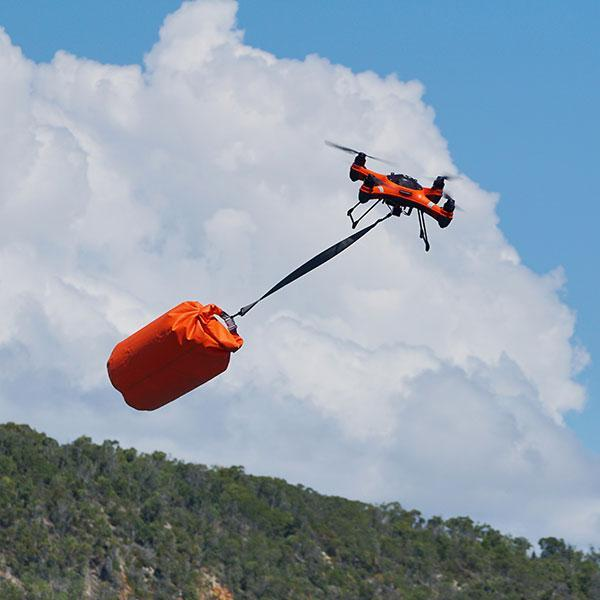
\includegraphics[width=0.45\linewidth]{real_suspended_payload_example.jpg}            
            \caption{A practical suspended payload used for search and rescue missions \cite{CompareCommander2020}}
            \label{fig:real_suspended_payload_example}
        \end{figure}

        \paragraph
        The transportation of various suspended payload configurations have been considered in literature.
        The classical suspended payload application involves a small payload suspended below the vehicle with rigid cable \cite{Erasmus2020, Slabber2020, Guerrero-Sanchez2017, Klausen2017, Ichikawa2018, DeAngelis2019a}. 
        \citet{Kotaru2017} considered a suspended payload system with an elastic cable modelled as a spring-damper system.
        \citet{Tang2015a} modelled the multirotor-payload system with a hybrid dynamical model to consider aggressive manoeuvres where the cable transitions from taut to slack.
        The transportation of payload loads with flexible cables have also been studied, where the cable is modelled as a set of serially-connected rigid links  \cite{Goodarzi2015, Goodarzi2014, Kotaru2018}. 
        Furthermore, the control of a group of multirotors transporting a single suspended payload have also been considered in various studies \cite{Lee2015, Sanalitro2020, Klausen2014, Goodarzi2015}.
        
        \paragraph
        From numerous examples in literature, it is clear that the control of multirotors with suspended payloads is a popular research topic.
        The cable-suspended payload configuration is very useful in situations where a multirotor cannot land, since the payload can be attached during hover.
        This configuration also has the advantage that a load can have an arbitrary shape or size as long as it has an attachment point for a cable.
        However, the suspended payload increases the degrees of underactuation of the system, which makes the control problem challenging \cite{Kotaru2018}.

        % ?? Fi author cite and [12-15] to rather [12,13,14,15]
\section{Control of a multirotor with a suspended payload}

    \paragraph
    A major drawback of transporting a cable-suspended payload is that the payload is free to swing during flight, which effects dynamics of the multirotor.
    Two main control strategies are applied in literature to stabilise a multirotor with a suspended payload, namely, trajectory generation and active vibration damping.
    Some methods apply a hybrid strategy that combine the two methods into a single control architecture.
    Trajectory generation methods involve determining multirotor trajectories that result in minimal oscillations or specific payload trajectories.
    Active vibration damping controllers involve feedback controllers that apply a control law to actively counteract the swing of the payload,

    \subsection{Trajectory generation}

        \paragraph
        Trajectory generation methods for suspended payload systems are based on open-loop control techniques.
        The objective of these techniques is to determine a trajectory in which the multirotor motion would induces a specific payload trajectory to reduce oscillations or avoid obstacels.
        Different trajectory generation methods have been applied successfully for suspended payload transportation.
        \citet{Zeng2019} and \citet{Tang2015b} applied differential flatness based trajectory planning methods for multirotors in obstacle-filled environments.
        Instead of only considering swing-reduction of the suspended payloads, these studies consider specific payload trajectories to avoid obstacles during aggressive motion.
        \citet{Xian2020} proposed an efficient online trajectory planning method without iterative optimizations.
        The swing-reduction performance of this method was also verified with experimental results.
        
        \paragraph
        Dynamic programming methods have also been implemented to generate swing-free trajectories with suspended payloads \cite{Starr2005, Palunko2012, Su2019}.
        These methods require accurate models of the plant dynamics and are sensitive to the accuracy of these models.
        \gls{RL} methods do not require prior models of the dynamics and have also been applied for swing-free trajectory generation \cite{Palunko2013, Faust2013}.
        \citet{Faust2013} implemented a \gls{RL} method for minimal swing trajectories which provides sufficient criteria to allow the learned policy to be transferred to a variety of different models, starting positions, and trajectories.
        Furthermore, this \gls{RL} trajectory generation method was verified with simulation and experimental results.

        % Look for newer literature. ??

        % ?? Maybe add this
        % \paragraph 
        % A drawback of \gls{MPC} and \gls{RL} methods is that they rely on cost functions with tuning weights and linear constraints for obstacle avoidance.
        % \citet{Silveira2020} addressed this problem by implementing a \gls{RRT} algorithm that does not rely on cost functions and constraints for collision-free trajectories with a suspended payload.
        % However, this approach does not provide an optimal solution, but rather finds any collision-free trajectory as a solution. 

        \paragraph
        Input shaping is another open-loop control method related to trajectory planning that has also been applied for minimal swing control of suspended payloads.
        This technique involves modifying a reference signal, usually with a set of timed impulses, to cancel oscillatory modes of the system \cite{Vaughan2008}.
        These techniques were originally designed for moving suspended payloads with gantry systems \cite{Smith1957, Starr1983}.
        Later, these input shaping techniques were also applied for reduced swing control of 
        helicopters \cite{Bisgaard2008, Potter2011} and 
        multirotors \cite{Homolka2017, Sadr2014b, Fielding2019} transporting suspended payloads.

        \paragraph
        \citet{Ichikawa2018a} compared different input shaping techniques for velocity control of a quadrotor with a suspended payload in simulations.
        The specific input shaping techniques considered were: \gls{ZV}, \gls{NZV}, \gls{EI}, and 2-hump \gls{EI}.
        These methods convolve a baseline input command with precisely timed impulses based on the length of the suspended cable. 
        Simulation results showed that the input shapers significantly decreased the residual payload oscillations compared to a baseline velocity controller.
        It was also highlighted that \gls{EI} and 2-hump \gls{EI} were more robust to cable length uncertainty than \gls{ZV} and \gls{NZV}.

        \paragraph
        \citet{Slabber2020} applied a notch filter to reduce the cable-suspended payload oscillation for velocity control of a multirotor in simulation.
        \citet{Slabber2020} considered a system with an unknown payload mass and cable length, estimated with \gls{RLS} and \gls{FFT} parameter estimators respectively.
        The natural frequency of the multirotor-payload system was calculated based on these estimates.
        The notch filter was applied to the velocity setpoint signal to suppress the frequency band containing this natural frequency. 
        To improve the robustness against parameter uncertainty, a wider frequency band could be used.
        It was shown in simulation that a notch filter attenuated the payload oscillations to near swing free motion even with large parameter estimation errors \cite{Slabber2020}.
    

    \subsection{Active vibration damping controllers}

        \paragraph
        Active vibration damping is a closed-loop control method where a feedback control law is applied that directly affects the payload states.
        Instead of finding a trajectory that reduces oscillations, these controllers track a given trajectory as close as possible while trying to reduce payload oscillations simultaneously.
        These controllers generally perform better than open-loop methods in the presence of parameter uncertainties and external disturbances \cite{Liang2021}.
         
        \paragraph
        backstepping control
        geometric control

        \paragraph
        Learning-based methods have also been proposed for multirotors with suspended payloads \cite{Hua2021}.
        \citet{Hua2021} develops a non-linear control strategy embedded with \gls{RL} for position control and simultaneous swing suppression.
        Experimental results showed that this method provided reliable swing suppression control in situations with model uncertainties, parameters drift, and external disturbances.

        \paragraph
        Erasmus

        \paragraph
        Slabber
        \citet{Slabber2020} also showed that the input shaper can be augmented for improved closed-loop active vibration damping control.
        \citet{Huo2019} also used combo of input shape and closed loop control ??.

        \paragraph
        \gls{MPC}

    
    % ?? Lit study: include different types of \gls{MPC}, e.g. DMC, MAC
    % ?? different types of models \cite{}, 
    % ?? See \cite{Garcia1989} for good example of different implementations with different models

    % ?? Table of literature
    % Unknown payloads
    % what is unknown

    % See data driven is scarece?
    % therefore data driven.
    % MPC is a good method of applying model

\section{Multirotor control with unknown dynamics}

    \paragraph
    Unknown states.
    Erasmus.
    Get more cites from erasmus.


    \subsection{Unknown parameters}
        
        \paragraph

    
    \subsection{Unknown models}
        
        \paragraph

        \paragraph
        RL

        \paragraph
        MPC with system identification

        \paragraph
        DMD

\section{Summary} 
        
    \paragraph
    Where does my work fit in.

    The major contribution of this work

% \section{System Design}
% Blok diagram
% komponente

}


